\section{Qafny: A High-level Quantum Language Admitted a Proof System}
\label{sec:qafny}

Here, we first introduce \qafny state equational properties and type system. Then, we discuss its semantics and proof system.

\subsection{State Equivalence, Type, and Sequence Rules}\label{sec:state}

\begin{figure}
{\footnotesize
{\hspace*{-6em}
\begin{minipage}[t]{0.35\textwidth}
\begin{center}
 \[
  \begin{array}{l@{~}cl}
  \tau & \sqsubseteq & \tau \\
  \tnort &\sqsubseteq& \tcht\\
  \thadt &\sqsubseteq& \tcht
    \end{array}
  \]
\end{center}
\subcaption{Subtyping}
  \label{fig:qafny-subtype}
\end{minipage}
\qquad
\begin{minipage}[t]{0.5\textwidth}
\begin{center}
   \[
   \begin{array}{l@{~}cl}
   q & \equiv_{\slen{q}} & q \\
  \ket{c} &\equiv_n& \sch{1}{ }{c}\\
  \shad{2^n}{n}{\alpha(r_j)} &\equiv_n& \sch{2^n}{\frac{\alpha(\sum_{k=0}^{n} r_k \cdot \tos{j}[k])}{\sqrt{2^n}}}{j}
    \end{array}
 \]
\end{center}
\subcaption{Quantum Value Equivalence}
  \label{fig:qafny-sequiv}
\end{minipage}
\hfill{}
\begin{minipage}[t]{0.8\textwidth}
\begin{center}
 \[
  \begin{array}{l @{~} c @{~} l l@{~}c @{~} l l @{~}c @{~} l l @ {~} c @{~} l}
\lambda &\equiv & \lambda
&
\qquad
x[n,n] & \equiv & \bot
&
\qquad
\bot \uplus \lambda & \equiv & \lambda
&
\qquad
x[n,m]\uplus\lambda & \equiv & x[n,j]\uplus x[j,m] \uplus\lambda
\\
&&&&&&&&&&&
\texttt{where}\;\;n \le j < m

    \end{array}
  \]
\end{center}
\subcaption{Session Equivalence}
  \label{fig:qafny-ses-equal}
\end{minipage}
\hfill{}
\hspace*{-5em}
\begin{minipage}[t]{0.475\textwidth}
\begin{center}
 \[
  \begin{array}{l@{~}c@{~}l}
    \sigma & \preceq & \sigma \\[0.2em]
  \{\bot:\tau\} \cup \sigma &\preceq& \sigma\\[0.2em]
   \{\lambda:\tau\} \cup \sigma &\preceq& \{\lambda:\tau'\} \cup \sigma\\
&&\texttt{where}\;\;\tau\sqsubseteq_{\slen{\lambda}}\tau' \\[0.2em]
  \{\lambda_1\uplus l_1 \uplus l_2 \uplus \lambda_2 :\tau\} \cup \sigma &\preceq& \{\lambda_1\uplus l_2 \uplus l_1 \uplus \lambda_2 : \tau\} \cup \sigma\\[0.2em]
  \{\lambda_1 :\tau\} \cup \{\lambda_2 :\tau\} \cup \sigma &\preceq& \{\lambda_1 \uplus \lambda_2 :\tau\} \cup \sigma \\[0.2em]
  \{\lambda_1 \uplus \lambda_2 :\tau\} \cup \sigma &\preceq& \{\lambda_1 :\tau\} \cup \{\lambda_2 :\tau\} \cup \sigma
\\
&&\texttt{where}\;\;\tau\neq\tcht
    \end{array}
  \]
\end{center}
\subcaption{Environment Equivalence}
  \label{fig:env-equiv}
\end{minipage}
\begin{minipage}[t]{0.475\textwidth}
\begin{center}
   \[
   \begin{array}{l@{~}c@{~}l}
    \varphi & \equiv & \varphi \\[0.2em]
  \{\bot:q\} \cup \varphi &\equiv& \varphi\\[0.2em]
   \{\lambda:q\} \cup \varphi &\equiv& \{\lambda:q'\} \cup \varphi\\
   &&\texttt{where}\;\;q\equiv_{\slen{\lambda}}q' 
   \\[0.2em]
  \{\lambda_1\uplus l_1 \uplus l_2 \uplus \lambda_2 :q\} \cup \varphi &\equiv& \{\lambda_1\uplus l_2 \uplus l_1 \uplus \lambda_2 : \texttt{mut}(q,\slen{\lambda_1})\} \cup \varphi\\[0.2em]
  \{\lambda_1 :q_1\} \cup \{\lambda_2 :q_2\} \cup \varphi &\equiv& \{\lambda_1 \uplus \lambda_2 :\texttt{mer}(q_1,q_2)\} \cup \varphi 
   \\[0.2em]
  \{\lambda_1 \uplus \lambda_2 :\varphi\} \cup \sigma &\equiv& \{\lambda_1 :\varphi_1\} \cup \{\lambda_2 :\varphi_2\} \cup \sigma
\\
&&\texttt{where}\;\;\texttt{spt}(\tau,\slen{\lambda_1})=(\varphi_1,\varphi_2)
    \end{array}
 \]
\end{center}
\subcaption{State Equivalence}
  \label{fig:qafny-stateequiv}
\end{minipage}
{\footnotesize
\[
\begin{array}{l}
\texttt{pmut}((c_1.i_1.i_2.c_2),n)=(c_1.i_2.i_1.c_2) \;\;\texttt{when}\;\slen{c_1}=n
\\[0.2em]
\texttt{mut}(\ket{c},n)=\ket{\texttt{pmut}(c,n)}
\\[0.2em]
\texttt{mut}(\frac{1}{\sqrt{2^m}}(q_1 \bigotimes (\ket{0}+\alpha(r_n)\ket{1}) \bigotimes (\ket{0}+\alpha(r_{n+1})\ket{1}) \bigotimes q_2),n)
\\
\qquad\qquad
=\frac{1}{\sqrt{2^m}}(q_1 \bigotimes (\ket{0}+\alpha(r_{n+1})\ket{1}) \bigotimes (\ket{0}+\alpha(r_n)\ket{1}) \bigotimes q_2)
\quad\texttt{when\;}\slen{q_1}=n
\\[0.2em]
\texttt{mut}(\sch{m}{z_j}{c_j},n)=\sch{m}{z_j}{\texttt{pmut}(c_j,n)}
\\[0.2em]
\texttt{mer}(\ket{c_1},\ket{c_2})=\ket{c_1.c_2}
\\[0.2em]
\texttt{mer}(\shad{2^n}{n}{\alpha(r_j)},\shad{2^m}{m}{\alpha(r_j)})=\shad{2^{n+m}}{n+m}{\alpha(r_j)}
\\[0.2em]
\texttt{mer}(\sch{n}{z_j}{c_j},\schk{m}{z_k}{c_k})=\schi{n*m}{z_j\cdot z_k}{c_j.c_k}
\\[0.2em]
\texttt{spt}(\ket{c_1.c_2},n)=(\ket{c_1},\ket{c_2}) \;\;\texttt{when}\;\slen{c_1}=n
\\[0.2em]
\texttt{spt}(q_1\bigotimes q_2,n)=(q_1,q_2) \;\;\texttt{when}\;\slen{q_1}=n
\end{array}
\]
}
  \caption{\qafny type/state relations. $\{\tos{j}|j\in[0,2^n)\}(2^n)$ defines a set $\{\tos{j}|j\in[0,2^n)\}$ with the emphasis that it has $2^n$ elements. $\{0,1\}$ is a set of two single element bitstrings $0$ and $1$. $\cdot$ is the multiplication operation, $\tos{j}$ turns a number $j$ to a bitstring, $\tos{j}[k]$ takes the $k$-th element in the bitstring $\tos{j}$, and $\ket{j}$ is an abbreviation of $\ket{\tos{j}}$. We use set union ($\cup$) to describe the state concatenation with the empty set operation $\emptyset$. $i$ is a single bit either $0$ or $1$. The $.$ operation is bitstring concatenation. Term $\Msum^{n*m}P$ is a summation formula that omits the indexing details.
Term $(\frac{1}{\sqrt{2^{n}}}\Motimes_{j=0}^{n}q_j) \bigotimes(\frac{1}{\sqrt{2^{m}}}\Motimes_{j=0}^{m}q_j)$ is equivalent to $\frac{1}{\sqrt{2^{n+m}}}\Motimes_{j=0}^{n+m}q_j$.}
  \label{fig:qafny-eq}
}
}
\end{figure}

As we suggested in \Cref{sec:shors}, quantum states have certain level of permutation symmetries. Essentially, quantum computation is implemented as circuits. In \Cref{fig:background-circuit-example}, if the first and second circuit lines and qubits are permuted, it is intuitive that the two circuit results are equivalence up to the permutation. Additionally, as indicated in \Cref{sec:shors}, we need quantum sessions to be split and regrouped sometimes. All these properties are formulated in \qafny as equational properties in \Cref{fig:qafny-eq} that rely on session rewrites, which can then be used as builtin libraries in the proof system. As one can imagine, the equational properties might bring nondeterminism in the \qafny implementation, such that the automated system does not know which equations to apply in a step. In dealing with the nondeterminism, we design a type system for \qafny to track the uses, split, and join of sessions, as well as the three state types in every transition step, so that the system knows exactly how to apply an equation.

\myparagraph{State Equivalence}
\Cref{fig:qafny-eq} shows the equivalence relations on types and states.
\Cref{fig:qafny-subtype} shows the subtyping relation such that $\tnort$ and $\thadt$ subtype to $\tcht$.
Correspondingly, the subtype of $\tnort$ to $\tcht$ represents the first line equation in \Cref{fig:qafny-sequiv}, where a $\tnort$ state is converted to a $\tcht$ form. Similarly, a $\thadt$ state can also be converted to a $\tcht$ state in the second line.
Additionally, \Cref{fig:qafny-ses-equal} defines the equivalence relations for the session concatenation operation $\uplus$: it is associative, identitive with the identity empty session element $\bot$.
We also view a range $x[n,n]$ to be empty ($\bot$), and a range $x[n,m]$ can be split into a two ranges in the session as $x[n,j] \uplus x[j,m]$. 

The main result to define state equivalence is to capture the permutation symmetry, split, and join of sessions introduced in \Cref{sec:shors}. The first rule describes the case for empty session, while the second rule in \Cref{fig:qafny-stateequiv} connects the quantum value equivalence to the state equivalence.
The third rule describes the qubit permutation equivalence by the \texttt{mut} function.
The fourth rule describes the join of two sessions in a state.
For the two sessions are of the type $\tnort$ and $\thadt$, a join means an array concatenation.
If the two sessions have $\tcht$ types, a join means a Cartesian product of the two basis states.
The final rule is to split a session, where we only allows the split of a $\tnort$ and $\thadt$ type state and their splits are simply array splits. Splitting a $\tcht$ type state is equivalent to qubit disentanglement, which is a hard problem and we need to upgrade the type system to permit certain types of such disentanglement. In \Cref{sec:newtype}, we upgrade the \qafny type system to a dependent type system to track the disentanglement of $\tcht$ type state.


\begin{figure}[t]
{
{\Small
  \begin{mathpar}
    \inferrule[TPar]{\sigma \preceq \sigma' \\ \Omega;\sigma' \vdash_g s \triangleright \sigma''}{\Omega;\sigma \vdash_g s \triangleright \sigma'' }

    \inferrule[TEXP]{\Omega[x\mapsto \cmode];\sigma\vdash_g s[n/x] \triangleright \sigma'}{\Omega;\sigma \vdash_g \sexp{x}{n}{s} \triangleright \sigma' }

    \inferrule[TMEA]{ \Omega(y)=\qmode{j} \\ \sigma(y) = \{y[0..j]\uplus\lambda\mapsto \tau \}
     \\\\ \Omega[x\mapsto \mmode];\sigma[\lambda \mapsto \tcht]\vdash_{\cmode} s \triangleright  \sigma'}{\Omega;\sigma \vdash_{\cmode} \sexp{x}{\smea{y}}{s} \triangleright \sigma' }

    \inferrule[TA-CH]{ FV(\Omega,\mu)=\lambda\\ \sigma(\lambda\uplus\lambda') = \tcht}{\Omega;\sigma \vdash_g \ssassign{\lambda}{}{\mu} \triangleright \{\lambda\uplus\lambda':\tcht\} }

    \inferrule[TDIS]{ FV(\Omega,l)=\lambda\\ \sigma(\lambda\uplus\lambda') = \tcht}{\Omega,\sigma \vdash_g \ssassign{\lambda}{}{\sdis} \triangleright \{l\uplus\lambda':\tcht\} }

    \inferrule[TSEQ]{\Omega;\sigma\vdash_g s_1 \triangleright\sigma_1
 \\\\\Omega;\sigma[\uparrow \sigma_1]\vdash_g s_2 \triangleright\sigma_2}{\Omega;\sigma \vdash_g \sseq{s_1}{s_2}\triangleright \;\sigma_2\cup\sigma_1|_{\not\in\dom{\sigma_2}} }

\inferrule[TIF]{ 
FV(\Omega,b)=\lambda\\
\lambda\cap FV(\Omega,s) =\emptyset 
\\\\
     \Omega;\sigma[\lambda \mapsto \tcht] \vdash_{\mmode} s \triangleright \{\lambda':\tcht\}} 
{\Omega;\sigma[\lambda \uplus \lambda' \mapsto \tcht] \vdash_g \sifq{b}{s} \triangleright \{\lambda\uplus \lambda':\tcht\} }


    \inferrule[TLOOP]{ \forall j\in[n_1,n_2)\;.\;\Omega;\sigma[\uparrow \sigma'[j/x]]\vdash_g \sifq{b}{s} \triangleright \sigma'[\texttt{S}\;j/x] }
                  {\Omega;\sigma \vdash_g \sqwhile{x}{n_1}{n_2}{b}{s} \triangleright \sigma'[n_2/x]}
  \end{mathpar}
}
{\footnotesize
\[
\sigma[\uparrow \sigma'] = \sigma[\forall \lambda:\tau \in \sigma'\;.\;\tau/\lambda]
\qquad
\sigma|_{\not\in\dom{\sigma'}}=\{\lambda:\tau|\lambda \not\in \dom{\sigma'}\}
\]
}
}
  \caption{\qafny type system. $\sigma(y)=\{\lambda\mapsto \tau\}$ produces the map entry $\lambda\mapsto \tau$ and the range $y[0..\slen{y}]$ is in $\lambda$. $\sigma(\lambda)=\tau$ is an abbreviation of $\sigma(\lambda)=\{\lambda\mapsto \tau\}$. $FV(\Omega, -)$ produces a session by union all qubits appearing in $-$ with the qubit group info in $\Omega$; see \Cref{sec:session-gen}.}
  \label{fig:exp-sessiontype}
\end{figure}

\myparagraph{Type Checking: A Quantum Session Type System}
In \qafny, typing is with respect to a \emph{kind environment} $\Omega$ and a \emph{finite type environment} $\sigma$,
which map \qafny variables to kinds and map sessions to types, respectively.
The typing judgment is written as $\Omega; \sigma\vdash_{g} s \triangleright \sigma'$,
which states that statements $s$ is well-typed under the context mode $g$ and environments $\Omega$ and $\sigma$,
the sessions representing $s$ is exactly the domain of $\sigma'$ as $\dom{\sigma'}$,
and $s$ transforms types for the sessions in $\sigma$ to types in $\sigma'$.
$\Omega$ describes the kinds for all program variables.
$\Omega$ is populated through \texttt{let} expressions that introduce variables,
and the \qafny type system enforces variable scope; such enforcement is neglected in \Cref{fig:exp-sessiontype} for simplicity.
We also assume that variables introduced in \texttt{let} expressions are all distinct through proper alpha conversions.
$\sigma$ and $\sigma'$ describe types for sessions referring to possibly entangled quantum clusters pointed to by quantum variables in $s$. 
$\sigma$ and $\sigma'$ are both finite and the domain of them contain sessions that do not overlap with each other; $\dom{\sigma}$ is large enough to describe all sessions pointed to by quantum variables in $s$,
while $\dom{\sigma'}$ should be the exact sessions containing quantum variables in $s$.
Selected type rules are given in \Cref{fig:exp-sessiontype}; the rules not mentioned are similar and listed in \Cref{sec:qafny-app}.

The type system enforces five invariants.  First, well-formed and context restrictions for quantum programs.
Well-formedness means that qubits mentioned in the Boolean guard of a quantum conditional cannot be accessed in the conditional body,
while context restriction refers to the fact that the quantum conditional body cannot create (\texttt{init}) and measure (\texttt{measure}) qubits. 
For example the $FV$ checks in rule \textsc{TIF} enforces that the session for the Boolean and the conditional body does not overlap.
Coincidentally, we utilize the modes ($g$, either $\cmode$ or $\mmode$) as context modes for the type system. 
Context mode $\cmode$ permits most \qafny operations. Once a type rule turns a mode to $\mmode$, such as in the conditional body in rule \textsc{TIF}, we disallow \texttt{init} and \texttt{measure} operations. For example, rules \textsc{TMEA} is valid only if the input context mode is $\cmode$.

Second, the type system tracks the basis state of every qubit in sessions. In rule \textsc{TA-CH}, we find that the oracle $\mu$ is applied on $\lambda$ belonging to a session $\lambda \uplus \lambda'$. The $\mu$ application preserves the session in $\tcht$ provided that the input type is turned to $\tcht$ type through rule $\textsc{TPar}$.
Third, the type system enforces equational properties of 
quantum qubit sessions through a partial order relation over type environments, including subtyping, qubit position permutation, merge and split quantum sessions through rule $\textsc{TPar}$.
Essentially, we can view two qubit arrays be equivalent if there is a bijective permutation on the qubit positions of the two.
To analyze a quantum application on a qubit array, if the array is arranged in a certain way, the semantic definition will be a lot more trivial than other arrangements. For example, in applying a quantum oracle to a session (rule \textsc{TMEA}), we fix the qubits that permits the $\mu$ operation to always live in the front part ($\lambda$ in $\lambda\uplus\lambda'$).
This is achieved by a consecutive application of the mutation rule ($\texttt{mut}$) in the partial order ($\preceq$) in \Cref{fig:env-equiv}, which casts the left type environment to the format on the right through rule \textsc{TPar}.

Fourth, the type system enforces that the $\cmode$ classical variables can be evaluated to values in the compilation time. \footnote{We consider all computation that only needs classical computer is done in the compilation time.}, while tracks $\mmode$ variables which represent the measurement results of quantum sessions. Rule \textsc{TEXP} enforces that a classical variable $x$ is replaced with its assignment value $n$ in $s$. The substitution statement $s[n/x]$ also evaluates classical expressions in $s$, which is described in \Cref{sec:qafny-app}.
Finally, the type system extracts the result type environment of a for-loop as $\sigma'[n_2/x]$ based on the extraction of a type environment invariant on the $i$-th loop step of executing a conditional $\sifq{b}{s}$ in rule \textsc{TLOOP}, regardless if the conditional is classical or quantum. 

\begin{figure*}[t]
{\small
\begin{tabular}{l}   
{\noindent\textcolor{blue}{\text{Predicate modeling:}}}\\

  \begin{mathpar}
    \inferrule[]{\Omega;\sigma\vdash \lambda \\  \models \varphi(\lambda) \mapsto q }{\Omega;\sigma,\varphi\models \lambda \mapsto q }

    \inferrule[]{ q\equiv_{\slen{q}} q' }{\models q \mapsto q' }

    \inferrule[]{ \sch{m}{z_j}{c_j} \subseteq \sch{m}{z'_j}{c'_j} \\ 
             \sch{m}{z'_j}{c'_j} \subseteq \sch{m}{z_j}{c_j} }{\models \sch{m}{z_j}{c_j} \mapsto \sch{m}{z'_j}{c'_j} }

    \inferrule[]{\sigma \bot \sigma' \\ \varphi \bot \varphi' 
      \\ \Omega;\sigma, \varphi \models P \\ \Omega;\sigma',\varphi' \models Q}
        {\Omega;\sigma \cup \sigma',\varphi \cup \varphi'\models P * Q }

    
  \end{mathpar}

\\[1em]
{\noindent\textcolor{blue}{\text{Sequence Semantic and Proof Rules:}}}\\[0.5em]


  \begin{mathpar}
    \inferrule[SSeq-1]{(\varphi,s_1) \longrightarrow (\varphi',s'_1)}{(\varphi,\sseq{s_1}{s_2})\longrightarrow (\varphi',\sseq{s'_1}{s_2}) }

    \inferrule[SSeq-2]{}{(\varphi,\sseq{\{\}}{s_2})\longrightarrow (\varphi,s_2) }

    \inferrule[PSeq]{
          \Omega;\sigma\vdash_g s_1 \triangleright \sigma' \\\\
       \fivepule{\Omega}{\sigma}{g}{P}{s_1}{R} \\ 
           \fivepule{\Omega}{\sigma[\uparrow \sigma']}{g}{R}{s_2}{Q}}
                {\fivepule{\Omega}{\sigma}{g}{P}{\sseq{s_1}{s_2}}{Q}}

  \end{mathpar}

\\[1em]
{\noindent\textcolor{blue}{\text{Pre-condition strengthening and Post-condition weakening Proof Rules:}}}\\[0.5em]

  \begin{mathpar}
    \inferrule[PConL]{
       (\Omega,\sigma,P) \Rightarrow (\Omega,\sigma',P') \\ \fivepule{\Omega}{\sigma'}{g}{P'}{s}{Q}}
                {\fivepule{\Omega}{\sigma}{g}{P}{s}{Q}}

    \inferrule[PConR]{\Omega,\sigma\vdash_g s_1 \triangleright \sigma'\\\\
          \fivepule{\Omega}{\sigma'}{g}{P}{s}{Q'} \\(\Omega,\sigma'',Q') \nRightarrow (\Omega,\sigma[\uparrow \sigma'],Q) }
                {\fivepule{\Omega}{\sigma}{g}{P}{s}{Q}}
  \end{mathpar}
\end{tabular}
}
{\footnotesize
\[
\begin{array}{l}
\\
(\Omega,\sigma,P) \Rightarrow (\Omega,\sigma',P') \triangleq \Omega,\sigma\vdash P \wedge \Omega,\sigma' \vdash P' \wedge \sigma \preceq \sigma' \wedge P \Rightarrow P'
\\[0.2em]
(\Omega,\sigma,Q) \nRightarrow (\Omega,\sigma',Q') \triangleq \Omega,\sigma\vdash Q \wedge \Omega,\sigma' \vdash Q' \wedge \sigma' \preceq \sigma \wedge Q \Rightarrow Q'
\ignore{
\\[0.2em]
\varphi \equiv \varphi' \wedge \varphi \models P \wedge \varphi' \models P' \Rightarrow (P \Leftrightarrow P') 
}
\end{array}
\]
}
\caption{Sequence and Consequence Rules}
\label{fig:exp-proofsystem-1}
\end{figure*}

\myparagraph{Taste of Semantic and Proof Rules: Sequence and Consequence}
We define the small step operational semantics of an \qafny program as a relation $(\Phi,s) \longrightarrow (\Phi',s')$, where $\Phi$ and $\Phi'$ are the pre- and post- states.

partial function
$\llbracket\rrbracket$ from
an instruction $\instr$ and input state $\varphi$ to an output state
$\varphi'$, written 
$\llbracket \instr \rrbracket\varphi=\varphi'$, shown in \Cref{fig:deno-sem}.


\begin{figure*}[t]
{\small

\begin{minipage}[t]{0.4\textwidth}
\subcaption{Application Analogy}
  \vspace{1cm}
  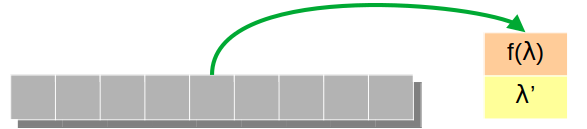
\includegraphics[width=\textwidth]{oracle}
  \label{fig:qafny-oracle-analog}
\end{minipage}
\hfill
\begin{minipage}[t]{0.5\textwidth}
\subcaption{App Function Modeling}
  \begin{mathpar}

    \inferrule[]{\forall j.\;\slen{c_{j1}}=n \\ \Omega;\sigma;\varphi\models \sch{m}{z_j}{\denote{\mu}(c_{j1}).c_{j2}\,\beta_j} \mapsto q}
          {\Omega;\sigma;\varphi\models \eth \;n.\denote{\mu}(\sch{m}{z_j}{c_{j1}.c_{j2}\,\beta_j}) 
              \mapsto q }
  \end{mathpar}
  \label{fig:qafny-mu-model}
\end{minipage}

\begin{minipage}[t]{\textwidth}
\subcaption{Semantic/Proof Rules}
  \begin{mathpar}
    \inferrule[SA-CH]{ \varphi(\lambda)=\{\lambda\uplus\lambda'\mapsto \sch{m}{z_j}{c_{j1}.c_{j2}\,\beta_j}\} \\\\ 
     \forall j.\; \slen{c_{j1}}=\slen{\lambda} \wedge \llbracket \mu \rrbracket c_{j1} = z'_j\ket{c'_{j1}} }{ (\varphi,\ssassign{\lambda}{}{\mu}) \longrightarrow (\varphi[\lambda\uplus\lambda'\mapsto \sch{m}{z'_j\cdot z_j}{c'_{j1}.c_{j2}\,\beta_j}],\{\}) }

    \inferrule[PA-CH]{\sigma(\lambda)=\{\lambda \uplus \lambda' \mapsto \tcht\}}
                {\fivepule{\Omega}{\sigma}{g}{P[\eth \;\lambda.\denote{\mu}(\lambda \uplus \lambda') / \lambda \uplus \lambda']}{\ssassign{\lambda}{}{\mu}}{P}}

    \inferrule[SH-N]{ FV(\emptyset,l)= \lambda \\ \varphi(\lambda)=\ket{c} }{ (\varphi,\ssassign{l}{}{\texttt{H}}) \longrightarrow (\varphi[\lambda\mapsto \shad{2^{\slen{c}}}{\slen{c}}{\alpha(\frac{1}{2^{c[j]}})}],\{\}) }

    \inferrule[PH-N]{FV(\Omega,l)=\lambda \\ \sigma(\lambda)=\tau}
                {\fivepule{\Omega}{\sigma}{g}{P[\eth \;\lambda.\denote{\texttt{H}}(\lambda) / \lambda]}{\ssassign{l}{}{\texttt{H}}}{P}}

  \end{mathpar}
  \label{fig:qafny-oracle-rules}
\end{minipage}
}
\caption{Oracle application and state preparation rules. $\eth$ is an array map operation, where $\eth \;\lambda.\denote{\mu}(\lambda \uplus \lambda')$ means that for every basis state in the state of $\lambda \uplus \lambda'$, we apply $\denote{\mu}$ to $\lambda$ part of session. }
\label{fig:exp-proofsystem-2}
\end{figure*}

\myparagraph{State Preparation and Oracle Application Rules}\label{sec:oracle-state}
The \qafny state preparation $\ssassign{l}{}{op}$ and oracle application $\ssassign{\lambda}{}{\mu}$ operations
are analogized to classical array map operation as indicated by the image on top of \Cref{fig:exp-proofsystem-2}, in which we have a session $\lambda\uplus \lambda'$, for each element $z_j\ket{c_{j1}.c_{j2}\,\beta_j}$ in the $\tcht$ type state, managed as an array having the form $\sch{m}{z_j}{c_{j1}.c_{j2}\,\beta_j}$ and $c_{j1}$ are the basis state for the $\lambda$ positions, we apply $\mu$ on the $c_{j1}$ part, which is described in the semantic rule \textsc{SA-CH}. Rule \textsc{PA-CH} describes the proof rule for capturing the array map analogy, where we substitute session $\lambda \uplus \lambda'$, representing the state before applying $\mu$, with the application of $\eth \;\lambda.\denote{\mu}$ on every element of $\lambda \uplus \lambda'$.
For example, in the loop body in \Cref{fig:shorqafny} line 8, we apply $\ssassign{y}{}{a^{2^j}y\;\%\; N}$ to a state $\{y[0..n]\} \mapsto \sch{2^{k\,\sminus\,1}}{\frac{1}{\sqrt{2^{k\,\sminus\,1}}}}{\tos{a^{\tos{j}}\;\%\;N} \,|\,\tos{j}.1}$ \footnote{The state is a equivalence state ($\{x[0..k],y[0..n]\} \mapsto \sch{2^k}{\frac{1}{\sqrt{2^k}}}{\tos{j}.\tos{a^{j}\;\%\;N}}$) of the masking session $x[0..j\,\splus\,1]$.}. The result is $\sch{2^{k\,\sminus\,1}}{\frac{1}{\sqrt{2^{k\,\sminus\,1}}}}{\tos{a^{\tos{j}.1}\;\%\;N} \,|\,\tos{j}.1}$ \footnote{We take the bitstring exponent formula as: $a^{c}= a^{\sum_{j}^{2^{c[j]}}}$. }.

Apparently, state preparation operations $\ssassign{l}{}{op}$ can also be described by an array map operation. The only tricky case is that applying an $\texttt{H}$ or $\texttt{QFT}$ gate in a basis state might result in generating more elements because of state preparations essentially turns a $\tnort$ state to become superposition. Here, we list the semantics and proof rules \textsc{SH-N} and \textsc{PH-N} for the case when dealing with $\tnort$ states. The other cases are listed in \Cref{sec:qafny-app}.

\begin{figure*}[t]
{\footnotesize
\begin{minipage}[t]{0.4\textwidth}
\subcaption{Conditional Analogy}
  \vspace{2cm}
  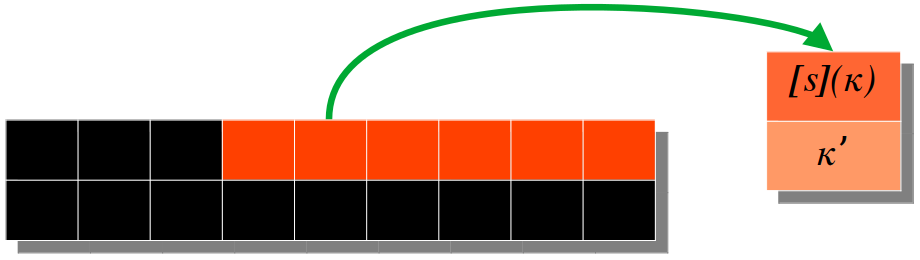
\includegraphics[width=1\linewidth]{conditional}

  \label{fig:qafny-con-analog}
\end{minipage}
\hfill
\begin{minipage}[t]{0.5\textwidth}
\subcaption{Mask/Unmask Function Modeling}
  \begin{mathpar}
    \inferrule[]{R \\ \Omega;\sigma;\varphi\models \theta \mapsto \sch{m}{z_j}{c_{j2}\,|c_{j1}\,\beta_j}}
          {\Omega;\sigma;\varphi\models \mathpzc{M}(b,\theta) 
              \mapsto \sch{m}{z_j}{c_{j1}.c_{j2}\,\beta_j}+q(\lambda,\neg b) }

    \inferrule[]{R
            \\\Omega;\sigma,\varphi\models \theta \mapsto \sch{m'}{z'_j}{c_{j1}.c'_{j2}\,\beta_j}+q(\lambda,\neg b)}
          {\Omega;\sigma,\varphi\models \mathpzc{U}(\neg b,\theta) \mapsto \sch{m}{z_j}{c_{j1}.c_{j2}\,\beta_j}+q(\lambda,\neg b)
  \\\\ \\ * \mathpzc{U}(b,\theta) \mapsto \sch{m'}{z'_j}{c'_{j2}\,|c_{j1}\,\beta_j} }
  \end{mathpar}

  \label{fig:qafny-mu-model}
\end{minipage}

{\begin{minipage}[t]{\textwidth}
\subcaption{Semantic/Proof Rules}
  \begin{mathpar}

\inferrule[SIF]{ R \\ FV(\emptyset,s)\subseteq \lambda'
          \\(\varphi[\lambda'\mapsto \sch{m}{z_j}{c_{j2}\,|c_{j1}\,\beta_j}],s) 
      \longrightarrow (\varphi[\lambda'\mapsto \sch{m'}{z'_j}{c'_{j2}\,|c_{j1}\,\beta_j}],s') } 
{(\varphi[\lambda\uplus\lambda'\mapsto \sch{m}{z_j}{c_{j1}.c_{j2}\,\beta_j}+q(\lambda,\neg b)],\sifq{b}{s}) \longrightarrow 
          (\varphi[\lambda\uplus\lambda'\mapsto \sch{m'}{z'_j}{c_{j1}.c'_{j2}\,\beta_j}+q(\lambda,\neg b)],\sifq{b}{s'}) }

    \inferrule[PIF]{\Omega;\{\lambda' : \tcht\} \vdash Q' \\ \fivepule{\Omega}{\sigma[\lambda' \mapsto \tcht]}{\mmode}{P[\mathpzc{M}(b,\lambda')/ \lambda \uplus \lambda']}{s}{Q * Q'}}
                {\fivepule{\Omega}{\sigma[\lambda \uplus \lambda' \mapsto \tcht]}{g}{P}{\sifq{b}{s}}{P[\mathpzc{U}(\neg b,\lambda \uplus \lambda')/\lambda \uplus \lambda')] * Q'[\mathpzc{U}(b,\lambda \uplus \lambda')/\lambda']}}

\mprset{flushleft}
    \inferrule[SLOOP]{ n_1 < n_2 }
                  {(\varphi,\sqwhile{j}{n_1}{n_2}{b}{s}) \longrightarrow \\\\ \quad (\varphi,\sseq{\sifq{b}{s}}{\sqwhile{j}{\texttt{S}\;n_1}{n_2}{b}{s})}}

    \inferrule[PLOOP]{n_1 < n_2\\ \fivepule{\Omega}{\sigma}{\mmode}{P(j)\wedge j \,\slt\, n_2}{\sifq{b}{s}}{P(\snext{j})} }
     {\fivepule{\Omega}{\sigma}{g}{P(n_1)}{ \sqwhile{j}{n_1}{n_2}{b}{s} }{P(n_2)} }

  \end{mathpar}

  \label{fig:qafny-mu-rules}
\end{minipage}
}
}
{\footnotesize
\[
\begin{array}{l}
\theta := q \mid \lambda
\\[0.2em]
q(\lambda,\neg b) = \schk{m}{z_k}{c_{k1}.c_{k2}\,\beta_k}
\;\;\texttt{where}\;\forall k.\;\slen{c_{k1}}=\slen{\lambda}\wedge \denote{\neg b[c_{k1}/\lambda]}
\\[0.2em]
R = FV(\emptyset,b)=\lambda \wedge \forall j.\; \slen{c_{j1}}=\slen{\lambda}\wedge\denote{b[c_{j1}/\lambda]}
\end{array}
\]
}
\caption{Semantic and Proof Rules for Conditionals and For-loops. $\theta$ is either a session or a quantum state. $\mathpzc{M}$ is the mask function and $\mathpzc{U}$ is the unmask function. }
\label{fig:exp-proofsystem-3}
\end{figure*}

\myparagraph{Rules for Conditionals and For-Loops}\label{sec:conditionals}
\Cref{fig:qafny-con-analog} describes the analogy of quantum conditionals in \qafny, which are partial map functions that only apply applications on the marked red parts and mask the marked black parts.
It contains two level of masking. For each basis state element in a state with session $\lambda_b\uplus \lambda_a$, it masks the $\lambda_b$ part of the state, i.e., if the state has the form: $\sch{m}{z_j}{c_{j1}.c_{j2}\beta_j}$ with $\slen{c_{j1}} = \slen{\lambda_b}$, we mask the $c_{j1}$ part by pushing it to a masked stack as $\sch{m}{z_j}{c_{j2}\,|\,c_{j1}\,\beta_j}$, which is described in preparing the pre-state of the upper-level transition in rule \textsc{SIF} (\Cref{fig:qafny-mu-rules}).
The second level of masking happens in selecting elements in the state by checking the Boolean condition $b$ on them.
The $R$ condition in rule\textsc{SIF} finishes such task for us.
Here, we split the state into two parts as $\sch{m}{z_j}{c_{j1}.c_{j2}\,\beta_j}+q(\lambda,\neg b)$, where the first part are all basis states satisfying $b$ since if we replace the variables in $b$ with $c_{j1}$, the evaluation $\denote{b[c_{j1}/\lambda]}$ returns true, while the second part $q(\lambda,\neg b)$ contains all basis states evaluated to false.
After the masking, we apply the application $s$ on each element in the selected states, install the results ($z'_j$ and $c'_{j2}$ back to the unmasked state, and result in $\sch{m'}{z'_j}{c_{j1}.c'_{j2}\,\beta_j}+q(\lambda,\neg b)$.
The result state number $m'$ might be different from the pre-state number $m$ because applications in $s$ might increase the state numbers such as applying a quantum diffusion operation.

To design a proof rule for such partial map, we develop the mask ($\mathpzc{M}$) and unmask ($\mathpzc{U}$) operations (\Cref{fig:qafny-mu-model}), both take a Boolean expression $b$ and a quantum state as the argument. $\mathpzc{M}$'s modeling materializes the masking mechanism above. For a state $\sch{m}{z_j}{c_{j1}.c_{j2}\,\beta_j}+q(\lambda,\neg b)$, we preserve the basis states satisfying $b$, as shown in the predicate $R$, remove the unsatisfied basis states $q(\lambda,\neg b)$, and push the bases $c_{j1}$ to state stacks.
Here, we do not need to input $\mathpzc{M}$ the session associated with $c_{j1}$, because we can learn it through $b$.
In the pre-condition manipulation of rule \textsc{PIF} (\Cref{fig:qafny-mu-rules}), we substitute $\lambda \uplus \lambda'$ with $\mathpzc{M}(b,\lambda')$. During the process, the type for the session in $\sigma$ is changed from $\lambda \uplus \lambda'$ in the bottom to $\lambda'$ in the upper level.
The unmask function $\mathpzc{U}$ assembles the result state of applying $s$ to the masked $\lambda$ state with the other parts hidden in the unmasked state (the part marked black in \Cref{fig:qafny-con-analog}). Function $\mathpzc{U}$ is usually appeared to be a pair with both $b$ and $\neg b$. In the post-condition manipulation, we substitute $\lambda \uplus \lambda'$ with $\mathpzc{U}(\neg b,\lambda \uplus \lambda')$ in $P$, representing the unchanged and masked state, substitute $\lambda'$ with $\mathpzc{U}(b,\lambda \uplus \lambda')$ in $Q'$, representing the result of applying $s$ on the unmasked part, and assemble them together through the separation operation $*$.
$\mathpzc{U}$'s modeling in \Cref{fig:qafny-mu-model} captures the assemble procedure by merging two $\mathpzc{U}$ constructs together.

Rules \textsc{SLOOP} and \textsc{PLOOP} are the semantic and proof rules for a for-loop, which is a repeat operation of conditionals in \qafny. The $P(j)$ is a loop invariant with $j$ being a variable. The case for $n_1 \ge n_2$ is given in \Cref{sec:newtype}. As an example, we show the proof for a loop-step in \Cref{fig:shorqafny}.

{\footnotesize
  \begin{mathpar}
\mprset{flushleft}
\inferrule[]{
   \inferrule[]
   { \inferrule[] {
    \fivepule{\Omega}{\sigma_2}{\mmode}{X(\snext{j}) * \{y[0..n]\}\mapsto C(j).1}{ s }{X(\snext{j}) * \{y[0..n]\}\mapsto C'(j).1} }
  { \fivepule{\Omega}{\sigma_2}{\mmode}{X(\snext{j}) * \mathpzc{M}(b,\{y[0..n]\})\mapsto 0.C(j)+1.C(j)}{ s }{X(\snext{j}) * \{y[0..n]\}\mapsto C'(j).1} } }
   {  \Omega,\sigma_1\vdash_{\mmode} \{X(\snext{j}) * \{x[0..\snext{j}],y[0..n]\}\mapsto 0.C(j)+1.C(j)\} \sifq{x[j]}{s}
     \\\\\qquad\qquad \{ X(\snext{j}) * \mathpzc{U}(\neg x[j],\{x[0..\snext{j}],y[0..n]\})\mapsto 0.C(j)
          * \mathpzc{U}(x[j],\{x[0..\snext{j}],y[0..n]\})\mapsto C'(j).1\}
     } } {
\fivepule{\Omega}{\sigma}{\mmode}{X(j) * \{x[0..j],y[0..n]\}\mapsto C(j)}{ \sifq{x[j]}{s} }{X(j\,\sminus\,1) * \{x[0..\snext{j}],y[0..n]\} \mapsto 0.C(j)+1.C'(j)} }
  \end{mathpar}
{\hspace*{-1.5em}
$\begin{array}{l}
X(j)=\shad{2^{n \,\sminus\,  j}}{n \,\sminus\, j}{}
\quad
C(j)=\sch{2^k}{\frac{1}{\sqrt{2^k}}}{\tos{j}^{k}.\tos{a^{\tos{j}^k}\;\%\;N}}
\quad
i.C(j)=\sch{2^{\snext{k}}}{\frac{1}{\sqrt{2^{\snext{k}}}}}{\tos{j}^k.i.\tos{a^{\tos{j}^k}\;\%\;N}}
\\
C'(j).i=\sch{2^{\snext{k}}}{\frac{1}{\sqrt{2^{\snext{k}}}}}{\tos{a^{\tos{j}^k.1}\;\%\;N}\,|\,\tos{j}^k.i}
\qquad
i.C'(j)=\sch{2^{\snext{k}}}{\frac{1}{\sqrt{2^{\snext{k}}}}}{\tos{j}^k.i.\tos{a^{\tos{j}^k.1}\;\%\;N}}
\\
\sigma_1=\{x[0..n\,\sminus\,\snext{j}] \mapsto \thadt, \{x[0..\snext{j}],y[0..n]\} \mapsto \tcht \}
\quad
\sigma=\{x[0..n\,\sminus\,\snext{j}] \mapsto \thadt, y[0..n] \mapsto \tcht \}
\quad
s=\ssassign{y}{}{a^{2^j}y\;\%\; N}
\end{array}$
}
}

The proof is built from bottom up. We first cut the $\thadt$ type state into two sessions ($x[0..n\,\sminus\,\snext{j}]$ and $x[j]$), join $x[j]$ with session $\{x[0..j],y[0..n]\}$, and double the state elements to be $0.C(j)+1.C(j)$, which is proved by applying the consequence rules. Notice that the type environment is also transitioned from $\sigma$ to $\sigma_1$.
By the same strategy of the $\mathpzc{U}$ rule in \Cref{fig:qafny-mu-model}, we combine the two $\mathpzc{U}$ terms into the final result. 
The second step applies rule \textsc{PIF} to substitute session $\{x[0..\snext{j}],y[0..n]\}$ with the mask construct $\mathpzc{M}(b,\{y[0..n]\})$ in the pre-condition and create two $\mathpzc{U}$ terms in the post-condition. The step on the top applies the modulo multiplication on every element in the masked state $\mapsto C(j).1$ by rule \textsc{PA-CH}.

\begin{figure*}[t]
{\footnotesize
\begin{minipage}[t]{0.4\textwidth}
\subcaption{Measurement Analogy}
  \vspace{0.5cm}
  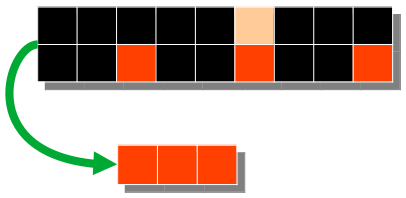
\includegraphics[width=1\linewidth]{measure}

  \label{fig:qafny-mea-analog}
\end{minipage}
\hfill
\begin{minipage}[t]{0.5\textwidth}
\subcaption{Measurement Modeling}
  \begin{mathpar}
    \inferrule[]{\Omega;\sigma;\varphi\models \theta \mapsto \theta'}
          {\Omega;\sigma;\varphi\models \mathpzc{F}(x,n,\theta) \mapsto \mathpzc{F}(x,n,\theta') }

    \inferrule[]{\slen{c}=n \\
           \Omega;\sigma;\varphi\models \theta \mapsto 
                      \sch{m}{\frac{z_j}{\sqrt{r}}}{c_{j}} \wedge x = (r,\tov{c})}
          {\Omega;\sigma,\varphi\models \mathpzc{F}(x,n,\theta) \mapsto \sch{m}{z_j}{c.c_{j}}+q(n,\neq c) }
  \end{mathpar}

  \label{fig:qafny-mea-model}
\end{minipage}

{\begin{minipage}[t]{\textwidth}
\subcaption{Semantic/Proof Rules}
  \begin{mathpar}

    \inferrule[SMea]{\varphi(y) = \{y[0..n]\uplus\lambda\mapsto \sch{m}{z_j}{c.c_{j}}+q(n,\neq c)\}}{(\varphi,\sexp{x}{\smea{y}}{s}) \longrightarrow (\varphi[\lambda \mapsto  \sch{m}{\frac{z_j}{\sqrt{r}}}{c_{j}}],s[(r,\tov{c})/x]) }

    \inferrule[PMea]{\fivepule{\Omega[x\mapsto \mmode]}{\sigma[\lambda\mapsto \tcht]}{\cmode}{P[\mathpzc{F}(x,n,\lambda)/y[0,n]\uplus\lambda]}{s }{Q} }
     {\fivepule{\Omega[y\mapsto \qmode{n}]}{\sigma[y[0,n]\uplus\lambda\mapsto \tcht]}{\cmode}{P}{\sexp{x}{\smea{y}}{s} }{Q} }

  \end{mathpar}

  \label{fig:qafny-mea-rules}
\end{minipage}
}
}
{\footnotesize
\[r= \sum_{k=0}^{m} \slen{z_k}^2
\qquad\qquad
q(n,\neq c) = \schk{m'}{z'_k}{c'.c'_{k}} \;\;\texttt{where}\;c'\neq c\]
}
\caption{Semantic and Proof Rules for Measurement. $\mathpzc{F}$ is the measurement function construct. $\tov{c}$ turns bitstring $c$ to an integer, and $r$ is the likelihood that the bitstring $c$ appears in a basis state. }
\label{fig:exp-proofsystem-4}
\end{figure*}

\myparagraph{Rules for Measurement}\label{sec:measurement}
As \Cref{fig:qafny-mea-analog} describes, quantum measurement is a two-step array filter: 1) each element in the state is partitioned into two parts, and we select a first part of an element as a key, as shown in the marked pink part; and 2) we create a new array state by removing all the first parts in the old state and collecting the elements whose first part is equal to the key.
The second step actually collects elements in a periodical manner as shown in the analogy in \Cref{fig:qafny-mea-analog}, where the marked red basis states appear in a periodical pattern in the whole state. This behavior is universally true for quantum operations, and many quantum algorithms utilize the periodical pattern of quantum computation.

In rule \textsc{SMea}, we pick an $n$-length bitstring $c$ as the marked pink key, and elect $m$ basis states $\sch{m}{z_j}{c.c_{j}}$ that has the key $c$. In the post-state, we update the remaining session $\lambda$ to $\sch{m}{\frac{z_j}{\sqrt{r}}}{c_{j}}$ with the adjustment of amplitude $\frac{1}{\sqrt{r}}$, and replace the variable $x$ in the statement $s$ with the value $(r,\tov{c})$.
In designing the proof rule \textsc{PMea}, the operation $\mathpzc{F}(x,n,\lambda)$ is invented,
whose modeling is in \Cref{fig:qafny-mea-model}, to do exactly the two steps above by selecting an $n$-length prefix bitstring $c$ in a basis state, computing the probability $r$, and assigning $(r,\tov{c})$ to variable $x$.
Rule \textsc{PMea} in \Cref{fig:qafny-mea-rules} replaces the session $y[0..n]\cup \lambda$ in $P$ with the measurement result session $\mathpzc{F}(x,n,\lambda)$ and updates the type state $\Omega$ and $\sigma$. 

{\footnotesize
  \begin{mathpar}
\inferrule[]{
   \inferrule[]
   { \fivepule{\Omega[u\mapsto \mmode]}{\sigma[\lambda \mapsto \tcht]}{\mmode}{\mathpzc{F}(u,n,x[0..n])\mapsto C'}{ \{\} }{x[0..n] \mapsto D * E} }
   { \fivepule{\Omega}{\sigma}{\mmode}{\{y[0..n],x[0..n]\}\mapsto C'}{ \sexp{u}{\smea{y}}{\{\}} }{x[0..n] \mapsto D * E}
     } } {\fivepule{\Omega}{\sigma}{\mmode}{\{x[0..n],y[0..n]\}\mapsto C}{ \sexp{u}{\smea{y}}{\{\}} }{x[0..n] \mapsto D * E} }
  \end{mathpar}
{\hspace*{-1em}
$\begin{array}{l}
C=\sch{2^{n}}{\frac{1}{\sqrt{2^{n}}}}{\tos{j}.\tos{a^{j}\;\%\;N}}
\quad
C'=\sch{2^{n}}{\frac{1}{\sqrt{2^{n}}}}{\tos{a^{j}\;\%\;N}.\tos{j}}
\quad
\sigma=\{\{x[0..\snext{j}],y[0..n]\}:\tcht\}
\\
D=\smch{\frac{1}{\sqrt{s}}}{s}{t\,\splus\,k p}
\quad
E=p = \texttt{ord}(a,N)
\wedge
u=(\frac{s}{2^n},a^{t}\;\%\;N)
\wedge
s=\texttt{rnd}(\frac{2^n}{p})
\end{array}$
}
}

For an instance, we show a proof fragment above for the partial measurement in line 11 in \Cref{fig:shorqafny}.
The bottom two lines are to modify the array group order of the session from 
$\{y[0..n],x[0..n]\}$ to $\{x[0..n],y[0..n]\}$ through the consequence rule of state equivalence.
The second line proof, applies rule $\textsc{PMea}$ by replacing session $\{x[0..n],y[0..n]\}$ with $\mathpzc{F}(u,n,x[0..n])$.
On the top statement, the pre- and post-conditions are equivalent, because of the periodical aspects in quantum computing.
In session $\{y[0..n],x[0..n]\}$, group $y[0..n]$ stores the basis state $\tos{a^{j}\;\%\;N}$, which contains value $j$ that represents the basis states for group $x[0..n]$. Selecting a basis state $a^{t}\;\%\;N$ also filters the $j$ in $x[0..n]$, which refers to any values $j$ having the relation $a^{j}\;\%\;N=a^{t}\;\%\;N$. Notice that modulo multiplication is a periodical function, which means that the relation can be rewritten $a^{t+kp}\;\%\;N=a^{t}\;\%\;N$, such that $p$ is the period order. Thus, the $x[0..n]$ state is rewritten as a summation of $k$: $\smch{\frac{1}{\sqrt{s}}}{s}{t\,\splus\,k p}$. The probability of selecting $\tos{a^{j}\;\%\;N}$ is $\frac{s}{2^n}$.
In \qafny, we set up additional axioms for representing these periodical manners, which is why the pre- and post-condition equivalence is granted.

\begin{figure*}[t]
{\footnotesize
\begin{minipage}[t]{0.35\textwidth}
\subcaption{Diffusion Analogy}
  \vspace{0.5cm}
  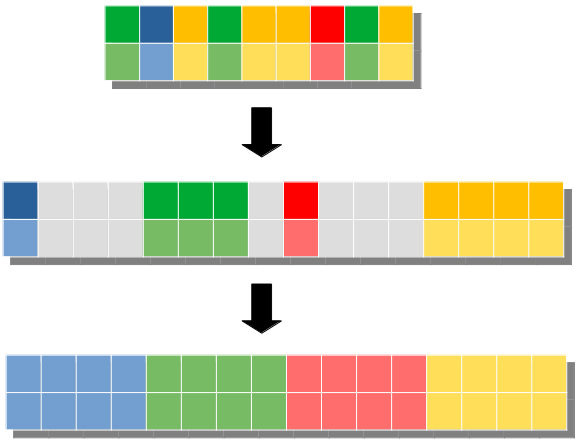
\includegraphics[width=1\linewidth]{diffuse}

  \label{fig:qafny-dis-analog}
\end{minipage}
\hfill
\begin{minipage}[t]{0.6\textwidth}
\subcaption{Diffusion Modeling}
  \begin{mathpar}
    \inferrule[]{\Omega;\sigma;\varphi\models \theta \mapsto \theta'}
          {\Omega;\sigma;\varphi\models \mathpzc{D}(n,\theta) \mapsto \mathpzc{D}(n,\theta') }

    \inferrule[]{\Omega;\sigma;\varphi\models \theta\mapsto \mathpzc{D'}(n,\sch{n'}{z_{i}}{c_{i}})}
          {\Omega;\sigma;\varphi\models \mathpzc{D}(n,\theta) \mapsto \schii{n'}{z_{i}}{c_{i}} }

    \inferrule[]{\slen{\tos{j}}=n
   \\ \Omega;\sigma;\varphi\models \theta\mapsto \Msum_{j=0}^{m}\schk{2^n}{(2 z_{jk}\sum_{t=0}^{2^n}z_{jt} - z_{jk})}{\tos{k}.c_{jk}}}
          {\Omega;\sigma;\varphi\models \theta \mapsto \mathpzc{D'}(n,\Msum_{j=0}^{m}\schk{2^{n}}{z_{jk}}{\tos{k}.c_{jk}}) }
  \end{mathpar}

  \label{fig:qafny-dis-model}
\end{minipage}

{\begin{minipage}[t]{\textwidth}
\subcaption{Semantic/Proof Rules}
  \begin{mathpar}

    \inferrule[SDis]{FV(\Omega,l)=\lambda \\ \varphi(\lambda) = \{\lambda\uplus\lambda'\mapsto q\}}
      {(\varphi,\ssassign{l}{}{\sdis}) \longrightarrow (\varphi[\lambda\uplus\lambda' \mapsto \mathpzc{D}(\slen{\lambda},q)],\{\}) }

    \inferrule[PDis]{ FV(\Omega,l)=\lambda\\\sigma(\lambda)=\{\lambda\uplus\lambda:\tcht\} }
     {\fivepule{\Omega}{\sigma}{g}{P[\mathpzc{D}(\slen{\lambda},\lambda\uplus\lambda')/\lambda\uplus\lambda']}{\ssassign{l}{}{\sdis} }{P} }

  \end{mathpar}

  \label{fig:qafny-dis-rules}
\end{minipage}
}
}
\caption{Semantic and Proof Rules for Diffusion Operations. $\mathpzc{D}$ models the diffusion operations. }
\label{fig:exp-proofsystem-5}
\end{figure*}

\myparagraph{Rules for Diffusion}\label{sec:diffuse}
Quantum diffusion operations ($\ssassign{l}{}{\sdis}$) reorient the amplitudes of basis states based on the basis state corresponding to $l$. They are analogized to an aggregate operation of reshape and mean computation, both appeared in many programming languages \footnote{Such as Python}.
The aggregate operation first applies a reshape, where elements are regrouped into a normal form, as the first agree of \Cref{fig:qafny-dis-analog}. More specifically, the diffusion modeling function $\mathpzc{D}(n,\theta)$ takes an $n'$-element state $\sch{n'}{z_{j}}{c_{j}}$ as the second rule in \Cref{fig:qafny-dis-model}. The $n$ number corresponds to the number of bits in the session potion matching $l$.
Then, we rearrange the state by a helper function $\mathpzc{D'}$ by extending the element number from $n'$ to $m*n$ with probably adding new elements that originally have zero amplitude (the marked white elements in \Cref{fig:qafny-dis-analog}), as the third rule in \Cref{fig:qafny-dis-model}.
Here, let's view a basis $c_{i}$ as a small-endian (LSB) number $\tov{c_{i}}$. The rearrangement of changing bases $c_{i}$ (for all $i$) to $\tos{k}.c_{jk}$ is analogized to rearranging a number $\tov{c_{i}}$ to become the form $2^n j+k$, with $k\in [0,2^n)$. 
Basically, the reshape step rearranges the basis states to be placed in a periodical counting sequence, with $2^n$ being the order.

The mean computation analogy (the second arrow in \Cref{fig:qafny-dis-analog}) takes every period in the reshaped state, and for each basis state, we redistribute the amplitude by the formula $(2 z_{jk}\sum_{t=0}^{2^n}z_{jt} - z_{jk})$.
In another word, for each period, given a basis state $k$, we sum all the amplitudes from $0$ to $2^n$ in the period as $z_{sum}$, then the redistributed amplitude for $k$ is $2 z_k z_{sum}-z_k$. 

Rule \textsc{SDis} is the semantics for diffusion $\ssassign{l}{}{\sdis}$, which applies the $\mathpzc{D}$ function to the session $\lambda \uplus \lambda'$, where $\lambda$ corresponds to the $l$'s session. Proof rule \textsc{PDis} replaces session $\lambda\uplus \lambda'$ with the application $\mathpzc{D}$ on the session.
Quantum diffusion operations are used in many algorithms, such as amplifying a basis state's amplitude value in Grover's search algorithm, or redistributing a possible path direction in quantum walk algorithm.
In these algorithms, the session piece that is diffused has either a small constant number of qubits or the whole session, meaning that the $n$ number in the $\mathpzc{D}$ function is either very small or equal to $\slen{\lambda \uplus \lambda'}$, as the whole session.
In either case, the summation formula in $\mathpzc{D}$'s modeling (\Cref{fig:qafny-dis-model}) can be rewritten as very few terms that facilitate the automated verification, which is exactly how we handle the diffusion operations in \qafny.
An example of Grover's search and quantum walk algorithm is given in \Cref{sec:arith-oqasm}.

\subsection{\qafny Metatheory}\label{sec:theorems}

The type system is sound and the proof system is proved to be sound and complete.


\myparagraph{Type Soundness}
We prove that well-typed \qafny programs are well defined; i.e., the
type system is sound with respect to the semantics. 
We begin by defining the session domain and state well-formedness.

\begin{definition}[Well-formed session domain]\label{def:well-formed-ses}\rm 
  A type environment $\sigma$'s session domain is \emph{well-formed}, written
  $\Omega \vdash \dom{\sigma}$, iff for every session $\lambda\in \dom{\sigma}$:
\begin{itemize}
\item $\lambda$ is disjoint unioned, i.e., for every two ranges $x[i..j]$ and $y[i'..j']$, $x[i..j]\cap y[i'..j']=\emptyset$.

\item For every range $x[i..j]\in\lambda$, $\Omega(x)=\qmode{n}$ and $[i,j) \subseteq [0,n)$.
\end{itemize}
\end{definition}

\begin{definition}[Well-formed \qafny state]\label{def:well-formed}\rm 
  A state $\varphi$ is \emph{well-formed}, written
  $\Omega;\sigma \vdash \varphi$, iff $\dom{\sigma} = \dom{\varphi}$, $\Omega\vdash\dom{\sigma}$, and:
\begin{itemize}
\item For every $\lambda \in \sigma$ such that $\sigma(\lambda) = \tnort$, $\varphi(\lambda)=\ket{c}$ and $\slen{c}=\slen{\lambda}$.

\item For every $\lambda \in \sigma$ such that $\sigma(\lambda) = \thadt$, $\varphi(\lambda)=\shad{2^n}{n}{\alpha(r_j)}$ and $\slen{\lambda}=n$.

\item For every $\lambda \in \sigma$ such that $\sigma(\lambda) = \tcht$, $\varphi(\lambda)=\sch{m}{z_j}{c_j\,\beta_j}$ and $\slen{\lambda}=\slen{c_j}$ for all $j$.
\end{itemize}
\end{definition}

The \qafny type soundness is stated as two theorems, type progress and preservation theorems. The proofs are done by induction on \qafny statements $s$ and mechanized in Coq. Type progress states that any well-typed \qafny program can take a move, while type preservation states that for any such move, the transitioned type and state are preserved and well-typed, respectively.

\begin{theorem}[\qafny type progress]\label{thm:type-progress-oqasm}\rm 
If $\Omega;\sigma \vdash_g s \triangleright \sigma'$ and $\Omega;\sigma \vdash \varphi$, then either $s=\{\}$, or there exists $\varphi'$ and $s'$ such that $(\varphi,s)\longrightarrow (\varphi',s')$.
\end{theorem}

\begin{theorem}[\qafny type preservation]\label{thm:type-preservation-oqasm}\rm 
If $\Omega;\sigma \vdash_g s \triangleright \sigma'$, $\Omega;\sigma \vdash \varphi$, and $(\varphi,s)\longrightarrow (\varphi',s')$, then 
there exists $\Omega'$ and $\sigma''$, $\Omega';\sigma'' \vdash_g s' \triangleright \sigma'$ and $\Omega';\sigma'' \vdash \varphi'$.
\end{theorem}

\myparagraph{Proof System Soundness and Completeness}
We prove that the \qafny proof system is well defined; i.e., any properties derived in the \qafny proof system for well-typed \qafny programs can be interpreted by the state transitions in the \qafny semantics.
In \qafny, there are three different state representations for a session $\lambda$ and two sessions can be joined into a large session.
Hence, given a statement $s$ and an initial state $\varphi$, the semantic transition $(\varphi,s) \longrightarrow^{*} (\varphi',\{\})$ might not be unique, in the sense that there might be different representations of $\varphi'$, due to the different state representations.
However, any $\tnort$ and $\thadt$ type state can be represented as a $\tcht$ type state, so that $\tcht$ type states can be viewed as the \emph{most general} state representation. We also have state equivalence relations defined for capturing the behaviors of session permutation, join and split. We define a \emph{most general state representation} of evaluating a statement $s$ in an initial state $\varphi$ below.

\begin{definition}[Most general \qafny state]\label{def:most-gen}\rm 
  Given a statement $s$, an initial state $\varphi$, kind environment $\Omega$, type environment $\sigma$, and context mode $g$, such that $\Omega;\sigma\vdash \varphi$, $\vdash_g s \triangleright \sigma^*$, $\Omega;\sigma[\uparrow \sigma^*]\vdash \varphi^*$, and $(\varphi,s) \longrightarrow^{*} (\varphi^*,\{\})$, $\varphi^*$ is the most general state representation of evaluating $(\varphi,s)$, iff for all $\sigma'$ and $\varphi'$, such that $\vdash_g s \triangleright \sigma'$, $\Omega;\sigma[\uparrow \sigma']\vdash \varphi'$ and $(\varphi,s) \longrightarrow^{*} (\varphi',\{\})$, $\sigma' \preceq \sigma^*$ and $\varphi' \equiv \varphi^*$.
\end{definition}

The \qafny proof system correctness is defined by the soundness and relatively completeness theorems below, which has been formalized and proved in Coq. The \qafny proof system only describes the quantum portion of the whole Qafny+Dafny system, and the quantum portion contains non-terminated programs. Hence, the soundness and completeness essentially refers to the partial correctness of the \qafny proof system and the total correctness is achieved by the Qafny+Dafny system through mapping \qafny to Dafny, i.e., a separation logic proof system. Essentially, the \qafny proof system correctness is defined in terms of programs being well-typed. The type soundness theorem suggests that any intermediate transitions of evaluating a well-typed \qafny program is also well-typed. Thus, we can conclude that the pre- and post- conditions of a program are modeled properly through the above modeling rules that rely on well-typed transition states.

\begin{theorem}[proof system soundness]\label{thm:proof-soundness}\rm 
For a well-typed program $s$, such that $\Omega;\sigma\vdash_g s \triangleright \sigma'$, $\fivepule{\Omega}{\sigma}{g}{P}{s}{Q}$, $\Omega;\sigma;\varphi\models P$, then there exists a state representation $\varphi'$, such that $(\varphi,s)\longrightarrow (\varphi',\{\})$ and $\Omega;\sigma[\uparrow\sigma'];\varphi'\models Q$, and there is a most general state representation $\varphi^*$ of evaluating $(\varphi,s)$ as $(\varphi,s)\longrightarrow (\varphi^*,\{\})$ and $\varphi' \equiv \varphi*$.
\end{theorem}

\begin{theorem}[proof system relative completeness]\label{thm:proof-completeness}\rm 
For a well-typed program $s$, such that $\Omega;\sigma\vdash_g s \triangleright \sigma'$, $(\varphi,s)\longrightarrow (\varphi',\{\})$ and $\Omega;\sigma\vdash \varphi$, there is most general state representation $\varphi^*$, such that $(\varphi,s)\longrightarrow (\varphi',\{\})$ and $\varphi' \equiv \varphi^*$ and $\Omega;\sigma\vdash_g s \triangleright \sigma^*$ and $\Omega;\sigma[\uparrow \sigma^*]\vdash \varphi^*$, and there are predicates $P$ and $Q$, such that $\Omega;\sigma;\varphi\models P$ and $\Omega;\sigma[\uparrow\sigma^*];\varphi^* \models Q$ and $\fivepule{\Omega}{\sigma}{g}{P}{s}{Q}$.
\end{theorem}




